\chapter{\MakeUppercase{suspended affixation and sentence processing}}

The previous chapter focused on SA and its environment. The results of the first experiment showed that SA is mostly reserved for inflectional suffixes and changes in the environment of SA affects its acceptability. The second experiment showed that performing SA has a non-additive cost that differs from an effect of conjuncts with mismatching features.

In this chapter my aim is to investigate how SA would interact with sentence processing. I first give the structural explanations for SA. I then present a structural ambiguity environment dependent on SA. I come up with an experiment design using the ambiguity environment and come up with hypotheses for the results. I end the chapter by reporting on the experiment results and analysis.


\section{Processing suspended affixation}

The overall interpretation from Chapter 2 indicates that SA is interpreted under two approaches. The first approach \citep{orgun1995flat,broadwell2008turkish, kornfilt2012revisiting} argues for structural sharing in different ways, the second approach \citep{erschler2018suspended,guseva2017postsyntactic} argues for an ellipsis analysis where exponents of morphemes are deleted\. In the following subsections I give what both approaches predict for the processing of SA.

\subsection{Lexical sharing}

In the lexical sharing approach, the suspended affix is affixed to the whole conjunction as illustrated in Figure \ref{fig:lexicalsharing}.

\begin{figure}[hbt!]
    \centering
    \begin{forest}
    [\ldots 
        [ConjP 
            [N1]
            [(conj)]
            [N2]] 
        [Affix]]
    \end{forest}
    \caption{Abstract representation of lexical sharing}
    \label{fig:lexicalsharing}
\end{figure}

In this approach, the feature values for the suffix are encoded in the whole conjunction as opposed to being only encoded in the second conjunct. Figure \ref{fig:suspension} shows a representation of SA in the expression \textit{kitap ve kalem-ler-i} `the books and the pencils'.

\begin{figure}[hbt!]
    \centering
    \begin{forest}
    [\ldots 
        [ConjP 
            [\begin{avm}
            \[\rm \textit{kitap} \\
            \[ {\Lex} & Book \\ 
            {\Cat} & {\Noun} \\
            {\Num} & {?} \\
            {\Case} & {?}
            \]
            \]
            \end{avm}]
            [\begin{avm}
            \[\rm \textit{kalem} \\
            \[ {\Lex} & Pencil \\
            {\Cat} & {\Noun} \\
            {\Num} & {?} \\
            {\Case} & {?}
            \]
            \]
            \end{avm}]]
        [\begin{avm}
        \[\rm \textit{-ler-i} \\
        \[{\Num} & {\Pl} \\
        {\Case} & {\Acc}
        \]
        \]
        \end{avm}]]
    \end{forest}
    \caption{SA of {\Pl} and {\Acc} in lexical sharing}
    \label{fig:suspension}
\end{figure}

The number feature has two values in Turkish: {\Sg} and {\Pl}. {\Pl} has an overt exponent \textit{-lAr} but the exponent for {\Sg} is $\emptyset$/zero. The exponent for {\Nom} in case feature is also $\emptyset$/zero. A basic lexical sharing approach would never have SA if zero exponents are used for feature encodings. The nouns would already have feature encodings with zero exponents. A remedy for this can be an update of the features, where the feature encodings in the affix override the default values signalled by zero exponent ($\emptyset$). In ambiguous cases of SA, such as the suspension of the {\Pl} and {\Poss}, this update depends on a choice to perform SA or not. In unambiguous cases of SA, such as the suspension of {\Case}, this update is not a choice but obligatory for a successful interpretation.


\subsection{Ellipsis}

In the ellipsis approach, the suspended affix is encoded for the second conjunct and the value of that affix is recovered for the first conjunct as illustrated in Figure \ref{fig:ellipsis}.

\begin{figure}[hbt!]
    \centering
    \begin{forest}
    [\ldots 
        [N1, name=n1]
        [N2-Affix, name=n2]]
    \draw[thick,dashed, ->] (n2) to[out=south east, in=south] node[midway, fill=white]{recover}(n1);    
    \end{forest}
    \caption{Abstract representation of ellipsis analysis}
    \label{fig:ellipsis}
\end{figure}

In this approach, the feature values of the suffix are first encoded to the conjunct it is attached to. Later, the values for that suffix are encoded for the first conjunct. Figure \ref{fig:suspension2} illustrates the ellipsis analysis for SA of {\Pl-\Acc} in \textit{kitap ve kalem-ler-i} `the books and the pencils'. 

\begin{figure}[hbt!]
    \centering
    \begin{forest}
    [\ldots 
        [\begin{avm}
        \[ \rm \textit{kitap} \\
        \[ {\Lex} & Book \\
        {\Cat} & {\Noun} \\
        {\Num} & \sout{{\Sg}} {\Pl}\\
        {\Case} & \sout{{\Nom}} {\Acc}
        \]
        \]
        \end{avm}, name=y]
        [\begin{avm}
        \[\rm \textit{kalem-ler-i} \\
        \[ {\Lex} & Pencil \\
        {\Cat} & {\Noun} \\
        {\Num} & {\Pl} \\
        {\Case} & {\Acc} 
        \]
        \]
        \end{avm}, name=x
        ]]
        \draw[thick, dashed, ->] (x) to[out=south east, in=south east] node[midway,fill=white]{recover {\Pl}, {\Acc}} (y);
    \end{forest}
    \caption{SA of {\Pl} and {\Acc} in ellipsis}
    \label{fig:suspension2}
\end{figure}

The two approaches do not predict differences in the processing of SA. For both approaches to work, a process of updating feature values takes place. In the cases where SA is ambiguous this update depends on the parser's choice. On the simplex sentences, the SA of {\Case} is unambiguous. The unambiguous {\Case} SA is an incentive for both approaches to predict that SA of {\Case} is always carried out in a local environment where the first conjunct is encoded by zero ($\emptyset$) exponent. In this study, I investigate if the unambiguous {\Case} SA in simplex sentences have effects on ambiguous {\Case} SA in complex sentences. In the next section I introduce the ambiguous environment that depends on whether {\Case} SA takes place.

\subsection{Environment}

In Turkish, there is an ambiguity environment where the ambiguity depends on whether SA of {\Case} takes place. See (\ref{ambiguity}) for an example. The ambiguity depends on the SA of {\Acc}. If SA takes place, the nouns \textit{çocuk} `child' and \textit{kadın} `woman' form a conjunction and become the object of the embedded verb \textit{kurtar-} `to save'. If SA does not take place, the noun \textit{çocuk} `child' and the noun \textit{adam} `man' form a conjunction and become the subject of the main clause.

\begin{exe}
    \ex \label{ambiguity} 
    \gll çocuk ve kadın-ı kurtar-an adam ev-e gel-di. \\ 
    child {\And} woman-{\Acc} save-{\Fp} man home-{\Dat} come-{\Pst} \\
    \glt SA: `[the man who saved the child and the woman] came home.'\\*
    No SA: `[the child] and [the man who saved the woman] came home.'
\end{exe}

This means that the unambiguous {\Case} SA in a simplex sentence can be made to be ambiguous in a complex one. This ambiguity can be regulated by a pronoun as a disambiguator like in (\ref{disambiguation}).

\begin{exe}
\ex \label{disambiguation}
\gll kadın ve yolcu-yu kurtar-an adam {[onları/ birbirlerini]} uyar-dı. \\ 
woman {\And} passenger-{\Acc} save-{\Fp} man {them/ each\_other} warn-{\Pst} \\
\glt `the man who saved the passenger and the woman warned them.' \\*
`the woman and the man who saved the passenger warned each other.'
\end{exe}

In this environment, a pronoun \textit{birbirlerin-{\Case}} `each\_other' requires two antecedents that are both subjects. A main clause subject in Turkish requires {\Nom} as {\Case}. This means that the {\Case} value for the first conjunct should remain {\Nom} as encoded by the zero ($\emptyset$) exponent. This requires that no SA to take place. The other pronoun \textit{onlar-{\Case}} `them' requires a resolution of two antecedents that are the objects of the relativized verb. In this case, SA needs to take place for the pronoun to be processed grammatically. 


\section{Experiment 3}
The main aim in this experiment is to answer the following questions:
\begin{itemize}
    \item Do people keep performing {\Case} SA even when it is ambiguous?
    \item If so, does the parallelism between the conjuncts influence it?
\end{itemize}


\subsection{Hypotheses}

Now that the SA of {\Case} is made to be ambiguous, I present how the deterministic and probabilistic parsers can operate in this ambiguity environment. I first outline the two outcomes that the deterministic serial parser predicts, then I outline how the probabilistic serial parser can operate and what is predicts.


\subsection{Deterministic serial parser}

The two main principles of this parser is minimal attachment and late closure. The ambiguity environment depends on how the conjunction is formed. Specifically how {\Case} is taken into consideration when forming a conjunction. In an example like (\ref{prosconj}), the first word receives a {\Nom} value for {\Case} and by the time the conjoiner is reached the first conjunct is formed.

\begin{exe}
\ex \label{prosconj}
\begin{multicols}{2}
\begin{xlist}
\ex \gll adam ve \ldots \\ man[{\Nom}] {\And} \ldots\\ \glt `the man and \ldots'
\columnbreak
\ex \begin{forest}
[\ldots 
    [BP 
        [DP$_{\Nom}$] 
        [B]]
    [\ldots]]
\end{forest}
\end{xlist}
\end{multicols}
\end{exe}


If the conjunction continues with a noun that is not marked with the same {\Case}, there are two options to consider. The first one works as the following. The {\Case} value of the first conjunct determines the {\Case} value of the second because nouns marked with different cases can't be conjoined in Turkish. Once the second conjunct is designated to have {\Nom} as its {\Case} value, encountering a noun with a different {\Case} should result in positing an embedded clause and the different {\Case} marked noun to be interpreted within it. As illustrated in (\ref{conjparallel}). This amounts to maintaining late closure, because the second conjunct was designated to have {\Nom} as its case.

\begin{exe}
\ex \label{conjparallel}
\begin{forest}
[DP$_{\Nom}$ 
    [BP 
        [DP$_{\Nom}$]
        [B]]
    [DP$_{\Nom}$ 
        [XP 
            [DP$_{\neg\Nom}$]
            [X]]
        [\ldots]]]
\end{forest}
\end{exe}

A deterministic serial parser does not force the structure in (\ref{conjparallel}). That is a result of assuming that the parser keeps conjuncts parallel in their {\Case} value immediately after the conjoiner. If such a parallelism is not taken into account and {\Case} mismatches are only handled after a possible conjunction is formed, a different structure is predicted.

Let us assume that the parser is given a second conjunct that is not marked with {\Nom} as in (\ref{prosconj1}). The correct parsing of this structure requires a grammaticality filter. Once both conjuncts are encoded with their own {\Case} values, a filter of comparing the two and deciding whether or not the conjunction can be saved needs to take place. In (\ref{prosconj1}), the first conjunct is marked with {\Nom} which does not have an overt exponent. This enables the parser to perform SA. This amounts to keeping minimal attachment, even though it requires additional processes that are costly. The resulting conjunction is marked with the case of the second conjunct and the parsing continues with the embedded verb taking the conjunction as its argument.

\begin{exe}
\ex \label{prosconj1}
\begin{forest}
[DP$_{\neg\Nom}$ 
    [BP 
        [DP$_{\Nom\rightarrow\neg\Nom}$] 
        [B]]
    [DP$_{\neg\Nom}$]]
\end{forest}
\end{exe}

The specific environment I provided uses embedded sentences to establish an ambiguity of {\Case} SA. To achieve that, the noun after the conjoiner is followed by a relativized verb. If the structure in (\ref{conjparallel}) is adopted, the verb is interpreted only with the second noun. The head noun of the relative clause is marked with {\Nom}. This head noun becomes the second conjunct, satisfying {\Case} match with the first conjunct. If the structure in (\ref{prosconj1}) is adopted, the verb is interpreted with both nouns that come before it and the head noun of the relative clause becomes one noun that is not part of a conjunction.

As a result, a deterministic serial parser can predict either performing SA or not depending on the assumption of how a conjunction is formed. If the conjuncts are taken to be parallel in {\Case} immediately after the conjoiner, SA is not performed. If the {\Case} parallelism is a grammaticality filter after a potential conjunction is formed, SA is performed.


\subsection{Probabilistic serial parser}

As per the deterministic serial parser, the probabilistic one can also predict both outcomes of performing or not performing SA in ambiguous environments. This time however the difference does not rely on how the conjunction is formed, but it relies on the processes that would include and follow performing or not performing SA. Instead of a filter of grammaticality or syntactic interpretation, a race between the options is taken. Following from the representation of (\ref{prosconj}), the parser encounters the second conjunct that is not marked with {\Nom}. Performing or not performing SA are the two structural options.

Let us take the route of performing SA and consider the processes that it entails. For a parser to know that it is in an SA environment, it needs to compare the {\Case} values of both conjuncts to see if SA is even felicitous. This can be an operation initiated by the conjoiner even before the second conjunct is reached, as a constraint for building a grammatical structure. Once the comparison is made and the first conjunct is shown to have {\Nom} as its {\Case}, an operation of feature value update of the first conjoiner from {\Nom} to the {\Case} of the second conjunct takes place. Then a conjunction of the two nouns is formed and the verb after the second noun takes the conjunction as its argument. This amounts to performing SA. The processes are the comparison of the two conjuncts in their {\Case} values and updating the feature value of the first conjunct when permissible.


Taking the route of not performing SA requires other processes. When the second conjunct is encountered and it is marked with {\Case} other than {\Nom} a comparison of {\Case} with the first conjunct is made, as presumably initiated by the conjoiner and not by the second conjunct. Not performing SA requires positing an embedded clause that the second noun belongs to. The nature of the ambiguity is accomplished through using {\Acc}, {\Dat}, {\Loc}, and {\Abl}. All arguments with those {\Case} values require a verb to be interpreted under. Positing an embedded structure includes the processes of building a VP and a nominalization because the first conjunct is a noun and semantic equivalence is a constraint for conjunction. This means that not performing SA involves one process of positing an embedded sentence which would entail building a complex structure of a verb and a nominalization.

As a result, a probabilistic serial parser predicts a result compatible with performing SA over not performing SA under the assumption that it ranks the cost of positing an embedded structure higher than of performing SA. Performing SA is an update in feature values, but not performing SA is building up a complex structure.










\subsection{Participants}
The participants were 132 students from Boğaziçi University who are native speakers of Turkish. In exchange for their participation they received 1 point to their overall course score with the consent of the course's instructor.

\subsection{Materials}

I used the environment I introduced in the previous section and altered the disambiguation and parallelism between the conjuncts. I provide the template for an experimental item in (\ref{constemplate})(`W' stands for `word', abbreviated because of space limitations).

\begin{exe}
\ex \label{constemplate}
[1W] CONJ1 and CONJ2-{\Case} [2W] PRONOUN [1W] MainVerb
\end{exe}

The pronoun is the factor of Disambiguation with levels: Subject and Object. In Subject, \textit{birbirlerin-{\Case}} `each\_other' disambiguates towards a no SA reading. In Object, \textit{onlar-{\Case}} `{\Tpl}' disambiguates towards an SA reading. The factor Parallelism has two levels: Parallel and Non-parallel. In Parallel, the conjoiner is immediately followed by a noun. In Non-parallel, the conjoiner is followed by an adjective first and then a noun. In (\ref{exp3conditions}), I give partial sentences for all the experimental conditions.
\begin{exe}
\ex \label{exp3conditions}
\begin{xlist}
    \ex Subject, Parallel\\* 
    \gll {\ldots} [baron] ve [şövalye-yi {\ldots} kral] birbirlerini {\ldots} dinle-yecek. \\ 
    {\ldots} baron {\And} knight-{\Acc} {\ldots} king each\_other {\ldots} listen-{\Fut} \\
    \glt `{\ldots} [the baron] and [the king who {\ldots} the knight] will listen to each other {\ldots}'
    
    \ex Subject, Non-parallel\\* 
    \gll {\ldots} [baron] ve [cesur şövalye-yi {\ldots} kral] birbirlerini {\ldots} dinle-yecek. \\ 
    {\ldots} baron {\And} bold knight-{\Acc} {\ldots} king each\_other {\ldots} listen-{\Fut} \\
    \glt `{\ldots} [the baron] and [the king who {\ldots} the bold knight] will listen to each other {\ldots}'
    
    \ex Object, Parallel\\* 
    \gll {\ldots} [baron ve şövalye-yi] {\ldots} kral onları {\ldots} dinle-yecek. \\ 
    {\ldots} baron {\And} knight-{\Acc} {\ldots} king {\Tpl} {\ldots} listen-{\Fut} \\
    \glt `{\ldots} the king who {\ldots} [the baron and the knight] will listen to them {\ldots}'
    
    \ex Object, Non-parallel\\*
    \gll {\ldots} [baron ve cesur şövalye-yi] {\ldots} kral onları {\ldots} dinle-yecek. \\ 
    {\ldots} baron {\And} bold knight-{\Acc} {\ldots} king {\Tpl} {\ldots} listen-{\Fut} \\
    \glt `{\ldots} the king who {\ldots} [the baron and the bold knight] will listen to them {\ldots}'
\end{xlist}
\end{exe}

After every sentence, a statement was presented and the participants judge if the statement was true or false depending on the sentence they read. The statement targeted the theta role assignments. It had two types. One that was only true with SA (Object conditions), meaning that the first conjunct held theta role relation with the embedded verb. The other was only true with no SA (Subject conditions), meaning that the first conjunct held theta role relation with the matrix verb. For the full list of sentences (items 1-40, fillers 101-180) and questions (items 1-40, fillers 101-180) see Appendix \ref{equivalanceitems}

\begin{exe}
\ex \label{exp3qtype}
\begin{xlist}
    \ex Subject true (no SA)\\* 
    \gll Baron kral-ı {\ldots} dinle-yecek. \\ 
    Baron[{\Nom}] king-{\Acc} {\ldots} listen-{\Fut}[{\Tsg}] \\
    \glt `The baron will listen to the king {\ldots}'

    \ex Object true (SA)\\* 
    \gll Kral baron-u ödüllendir-miş \\ 
    King[{\Nom}] baron-{\Acc} reward-{\Prf}[{\Tsg}] \\
    \glt `The king {\ldots} the baron.'
\end{xlist}
\end{exe}

\subsection{Procedure}

Participants were provided with a link to the experiment prompting them with a consent page. Upon giving consent, the participants went through 5 practice items and then they were prompted again for the beginning of the experiment. Each trial proceeded by the participants pushing the `space' key, for each key stroke a word at the center of the screen appeared and by each key stroke it was replaced with the following word in the sentence. After the sentence was read, the participants were presented with a statement that was either true or false according to the sentence they read. They professed their decision by pushing `Q' key for `yes' and `P' key for `no' on the keyboard. The experiment only recorded word reading times, responses, and response times. After the experiment was done, the participants were redirected to a separate page where they provided their student information to be relayed to the course's professor for the extra credit. This is kept separate of the experiment results, keeping participant information and experimental data anonymous.

\subsection{Results}

The results were recorded onto a csv file and imported into R \citep{team2013r} for data cleaning, aggregation, and analysis. The data consisted of 140714 data points. 1 subjects with accuracies lower than 70\% in filler items are excluded from the data. The trials which had a word with reading times outside 100-3000 milliseconds are considered as outliers and also excluded. These exclusions resulted in the loss of 8.17\% of the data. In Figure \ref{fig:exp3sentenceread}, I give the average reading times per word with a representative sentence.


\begin{knitrout}
\definecolor{shadecolor}{rgb}{0.969, 0.969, 0.969}\color{fgcolor}\begin{figure}[hbt!]

{\centering 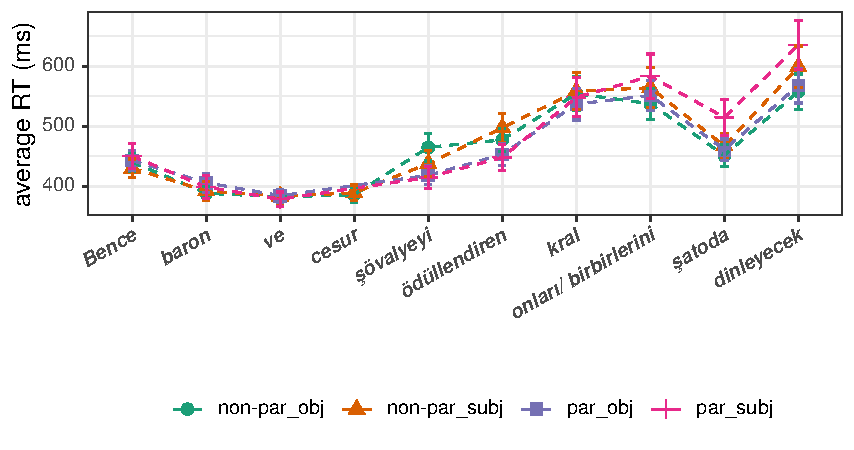
\includegraphics[]{experiments/equivalance/report/figure/exp3sentenceread-1.pdf} 

}

\caption[Average reading times of words for all experiment conditions by Disambiguation(Subject|Object) and Parallelism(Parallel|Non-parallel)]{Average reading times of words for all experiment conditions by Disambiguation(Subject|Object) and Parallelism(Parallel|Non-parallel)}\label{fig:exp3sentenceread}
\end{figure}


\end{knitrout}

The critical region in all the sentences is the Disambiguation word \textit{onlar-{\Case}} or \textit{birbirlerin-{\Case}}. The spillover region in all the sentences is the two words after the Disambiguation word. In the case of Figure \ref{fig:exp3sentenceread} it is the two words \textit{şatoda} `at the chateau' and \textit{dinleyecek} `will listen'. I give the average RTs of critical and spillover regions in Figure \ref{fig:exp3critandso}. On average Subject and Parallel conditions result in higher RTs.

\begin{knitrout}
\definecolor{shadecolor}{rgb}{0.969, 0.969, 0.969}\color{fgcolor}\begin{figure}[hbt!]

{\centering 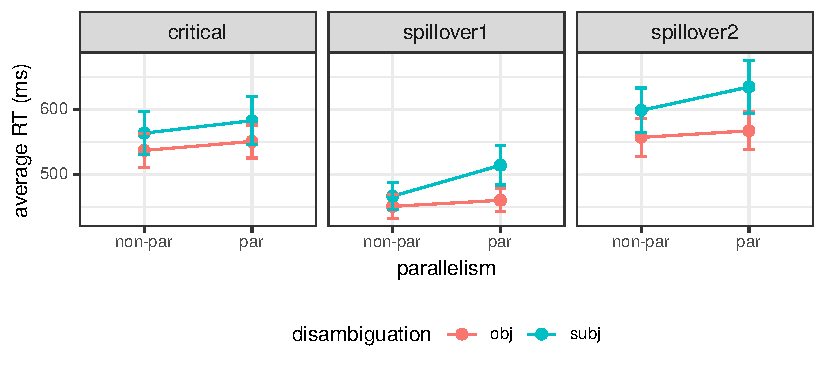
\includegraphics[]{experiments/equivalance/report/figure/exp3critandso-1.pdf} 

}

\caption[Third experiment, average reading times of critical and spillover regions by Disambiguation(Subject|Object) and Parallelism(Parallel|Non-parallel)]{Third experiment, average reading times of critical and spillover regions by Disambiguation(Subject|Object) and Parallelism(Parallel|Non-parallel)}\label{fig:exp3critandso}
\end{figure}


\end{knitrout}

For more inference in RTs in critical and spillover regions, I fit a regression model using brms package in R \citep{burkner2017brms}. I used sum contrasts for the predictors and controlled for the random effects for participant and experimental item. I give the results of the models in Figure \ref{fig:exp3critandsomodel}. The model results indicate that Subject and Parallel conditions have a main effect of increasing RTs. They are more pronounced in the spillover region.

\begin{knitrout}
\definecolor{shadecolor}{rgb}{0.969, 0.969, 0.969}\color{fgcolor}\begin{figure}[hbt!]

{\centering 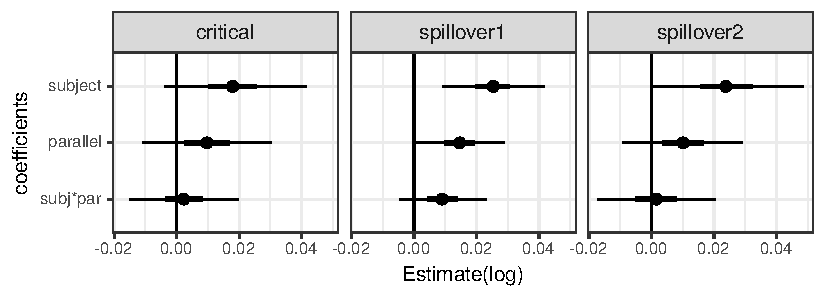
\includegraphics[]{experiments/equivalance/report/figure/exp3critandsomodel-1.pdf} 

}

\caption[Third experiment, model results of RTs for critical and spillover regions with the predictors Disambiguation(Subject|Object) and Parallelism(Parallel|Non-parallel)]{Third experiment, model results of RTs for critical and spillover regions with the predictors Disambiguation(Subject|Object) and Parallelism(Parallel|Non-parallel)}\label{fig:exp3critandsomodel}
\end{figure}


\end{knitrout}

In Figure \ref{fig:exp3accuracy}, I give participant accuracies grouped by experiment conditions and correct answer type. On average, participant accuracies are high in Object conditions and when the correct answer is `yes'. There is an interaction between the correct answer `no' and the Subject conditions where the accuracies are considerably lower.

\begin{knitrout}
\definecolor{shadecolor}{rgb}{0.969, 0.969, 0.969}\color{fgcolor}\begin{figure}[hbt!]

{\centering 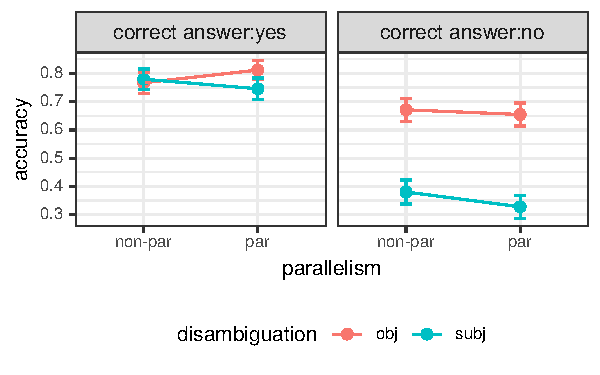
\includegraphics[]{experiments/equivalance/report/figure/exp3accuracy-1.pdf} 

}

\caption[Third experiment, average participant accuracy by Disambiguation(Subject|Object) and Parallelism(Parallel|Non-parallel)]{Third experiment, average participant accuracy by Disambiguation(Subject|Object) and Parallelism(Parallel|Non-parallel)}\label{fig:exp3accuracy}
\end{figure}


\end{knitrout}

For more inference in response accuracy, I fit a regression model using brms in R. This time, the correct answer type is added to the predictors. All predictors have sum contrasts and I controlled for random effects of subject and item. I give the model results in Figure \ref{fig:exp3accuracymodel}.

\begin{knitrout}
\definecolor{shadecolor}{rgb}{0.969, 0.969, 0.969}\color{fgcolor}\begin{figure}[hbt!]

{\centering 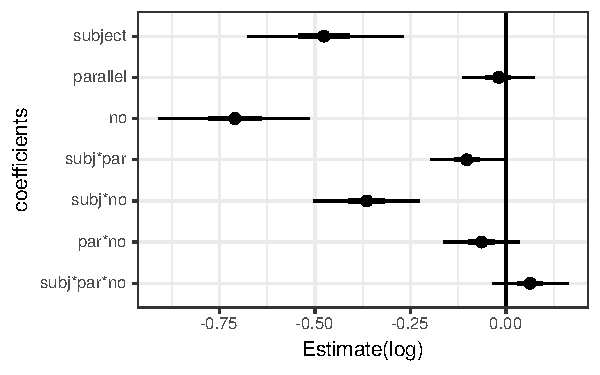
\includegraphics[]{experiments/equivalance/report/figure/exp3accuracymodel-1.pdf} 

}

\caption[Third experiment, model results for subject accuracies fit to responses with the predictors Disambiguation(Subject|Object), Parallelism(Parallel|Non-parallel), and Correct Answer(yes|no)]{Third experiment, model results for subject accuracies fit to responses with the predictors Disambiguation(Subject|Object), Parallelism(Parallel|Non-parallel), and Correct Answer(yes|no)}\label{fig:exp3accuracymodel}
\end{figure}


\end{knitrout}

\subsection{Analysis}

I evaluate the results of the experiment in two parts. In the first part, I analyze the changes in RTs. In the second part I analyze the changes in response accuracies. 

\subsubsection{Analysis of reading times}

Subject conditions result in higher RTs than Object conditions. This means that the parser have gone through a process that costs extra effort in Subject conditions. These conditions require having no suspension of {\Case}. Increase in Subject conditions means that the initial reading was compatible with an SA interpretation but it was changed. This indicates suspension taking place in local environments, no matter what the structural ambiguity in the sentence as a whole is. This is a Reanalysis effect directly related to SA and how the parser operates when it is possible to perform SA.


Parallel conditions display higher RTs than non-parallel conditions. There is no structural ambiguity that the effect can be attributed to. In both levels of Disambiguation, accessing a conjunction is required for establishing antecedents for the pronoun. There is an interaction between the levels Subject and Parallel in the first spillover word, suggesting an increase in difficulty. In Subject conditions, the conjunction needs to be accessed and then broken apart. After this operation, a new conjunction is formed. This first noun and the head noun of the relative clause are conjoined as subjects.


Parallel conditions do not have any contrast between the conjuncts whereas non-parallel conditions have the second conjunct modified by an adjective. This creates a contrast between the conjuncts. Marked conjuncts being more accessible for retrieval has been shown previously \citep{Hofmeister2014} and similarity effects for establishing dependencies are also attested (see \cite{Jager2017} for a review). In Subject conditions the conjunction to be broken apart needs to be retrieved, and the first noun needs to be taken out the conjunction. Addressing the correct noun in memory becomes harder in parallel conjuncts. This breaking process may be an effect of $dechunking$ \cite{martin2011direct}.


There is a main effect of Parallelism, relatively stable in all regions. It is more pronounced, as the interaction effect, in the first spillover word. I do not see an inherent reason for why parallel conjuncts increase difficulty. It is actually shown to facilitate processing in conjunctions \citep{frazier2000processing}, yet here it displays an opposite effect. The parallelism tested in \citep{frazier2000processing} is not a target to be broken apart or establishing antecedent relations with. 


The only thing common in the pronouns that are used for Disambiguation is their number marking. They are both marked {\Pl} but there is no plural noun among the possible antecedents. The pronoun number agrees with a complex number feature that takes the number of conjuncts instead of the number markings on nouns. Plural agreement is not obligatory in Turkish for conjoined nouns so there is no incentive to form a {\Pl} value for a conjunction when it is formed. I speculate that the easier it is to form a conjunction the harder it gets to address its parts for establishing a complex feature for number. This is the main effect that is observed in my experiment. Parallel conjuncts are easier to form, average reading differences on the second conjunct \textit{şövalyeyi} in Figure \ref{fig:exp3sentenceread} and a regression model with only Parallelism as the predictor (median log estimate -0.027, \%50 CI -0.032--0.021, \%95 CI -0.042--0.011) confirms the processing ease of parallel conjuncts. This makes it harder to access their parts in forming a complex feature for the conjunction since each of the conjuncts needs to be checked for the number feature. It even makes it harder to break the conjunction apart and form a new one.



\subsubsection{Analysis of response accuracies}

The participants were given a statement to judge depending on the sentence they read. This makes the statement a memory probe for which the participants search compatible readings in their memories. A match results in answering with `Yes' and a lack of finding a match results in answering with `No'. 

Subject conditions decrease participant accuracies overall. In Subject conditions, there was a point of Reanalysis. Overall decrease in Subject conditions mean that either the Reanalysis was not carried out even if it was, the statement was still judged erroneously. There is an interaction between the level Subject and `No' as the correct answer. This means that when the participants were supposed to answer with `No' in Subject conditions, they performed worse compared to Object conditions or `Yes' as the correct answer. This interaction can be attributed to matching the statement to a reanalyzed reading in the memory. When the statement is taken to be a memory probe, the participant had two readings formed, one that is actually true and one that was reanalyzed. The existence of both readings in the memory makes both statement types to have a match thereby decreasing accuracy further when the statement is indeed false. This is in line with the studies that show readings being addressable in memory \citep{christianson2001thematic,van2006activation,Slattery2013} even after Reanalysis.

When the statement was indeed false and the participants were supposed to answer with `No', they performed lower in general compared to the statements that were indeed true. When the statement is taken to be a memory probe for finding a match in memory, answering with `No' becomes the result of an exhaustive search that requires checking all available readings. This exhaustive operation might result in parser abandoning the search and give a random answer, possibly biased towards yes. Remember that not all statements are made about the theta role assignments and false statements only make up 1/4 of the questions. This reduces the chances of conditioning the parser for the task \citep{Swets2008,logavcev2016multiple}. 

Parallel conjuncts do not have a main effect and only have interaction effects with Subject and `No' as correct answer. It reduced accuracy in both. The main effect of increased difficulty in reading times seem to have effected Subject conditions more than they did Object conditions. It was shown that Subject and Parallel conditions had an interaction in the first word of the spillover. Subject conditions included a process of Reanalysis. The difficulty of breaking the conjunction combined with the Reanalysis might have proven too much for the parser, and lead to misparsing hence the interaction effect. In object conditions though, this increased difficulty did not lead to misparsing and that is why a main effect of Parallel seems to be lacking (although the median estimate and \%50 credible intervals are below zero indicating a relatively decrease in accuracy). All the effects of Subject and `No' as correct answer, and interaction with parallel decreasing accuracies are compatible with $good\,enough\,approach$ \citep{ferreira2001misinterpretations,ferreira2007good} that suggests language input is not strictly implemented during processing. Partially satisfied relations are taken to be enough if the required effort exceeds the resources that the parser is needed to allocate. 



\section{Discussion}

The second experiment showed that suspension of a suffix is costly, yet this experiment has shown that it is a preferred operation. A deterministic serial parser can predict this, as long as it filters possible conjunctions for {\Case} match and carry out any process necessary to satisfy it to keep the structure minimal. A probabilistic serial parser can predict this result as well, considering that suspension takes less processing resources (thereby time) than positing an embedded clause. The results further indicate that the participants did not fully interpret the sentences when the processing cost proved higher than expected.

In the experiment, the ambiguity environments did not use only {\Acc} to be reconstructed, there were examples of {\Dat}, {\Loc}, and {\Abl} in similar numbers. These can fall into different categories of {\Case} \citep{woolford2006lexical} and their category is only apperant when a verb is reached. Thereby {\Case} can play both a syntactic and a semantic role. If thematic roles are preemptively assigned by {\Case}, then the participants should have favored no SA reading. Some studies in German \citep{gorrell2000subject,schlesewsky2000subject,bader2000reanalyis} show that ambiguous {\Case} markings on arguments receive preferred readings of subject over object. The preferred reading is compatible with an SOV ordering just like the canonical word order in Turkish. None of those studies employ an example of {\Case} ambiguity in a conjunction where both the subject ({\Nom}) and the internal argument ({$\neg$\Nom}) {\Case} markings are available by means of SA. Another difference is that {\Case} is decomposable in Turkish, and no {\Case} marking is ambiguous. Even when the first conjunct was marked with {\Nom} and canonical word order being SOV in Turkish, the participants favored a reading that is incompatible with the {\Nom} or Subject interpretation. There is one crucial point in this experiment. To prevent information structure driven effects, I placed the nominative marked noun not in a sentence initial position, but following a speech act adverbial. This might have prevented the information like SOV word order to be used.


\section{Conclusion}

The results and the analysis indicate that people still perform SA of {\Case} even when it is made ambiguous. Conjunct parallelism do not regulate performing SA or not, but it effects the cost of Reanalysis. This experiment has shown that {\Case} information is overwritten for the sake of positing minimal structures, or structures that take less time to build. This means that the parser favors syntactically simple structures to morphologically complex operations.


The effects of {\Case} for processing ambiguities of conjunctions received very little attention in the literature. The only relevant study I could find was \cite{Traxler1996} where the {\Case} ambiguous `you' in English is contrasted to the unambiguous pronouns for predicting the attachment for c-selection ambiguous verbs like `recognize' that can have both a sentence and a noun as their internal argument. That study concludes in participants using {\Case} information rapidly and effectively. A similar but different story holds for this experiment, the {\Case} is updated in local environments of conjunction. Breaking this update is costly or even not done properly after a contradicting information is encountered.






